\section{Nondeterministic Finite Automata}

In this section we add a powerful and intriguing feature to finite automata.
This feature is called \textbf{nondeterminism}, and is essentially the ability to change states in a way that is only partially determined by the current state and input symbol. That is, we shall now permit several possible ``next states'' for a given combination of current state and input symbol. 

The automaton, as it reads the input string, may choose at each step to go into anyone of these legal next states; the choice is not determined by anything in our model, and is therefore said to be \textit{nondeterministic}. On the other hand, the choice is not wholly unlimited either; only those next states that are legal from a given state with a given input symbol can be chosen. 

\newpage

\begin{figure}[ht!]
  \centering
  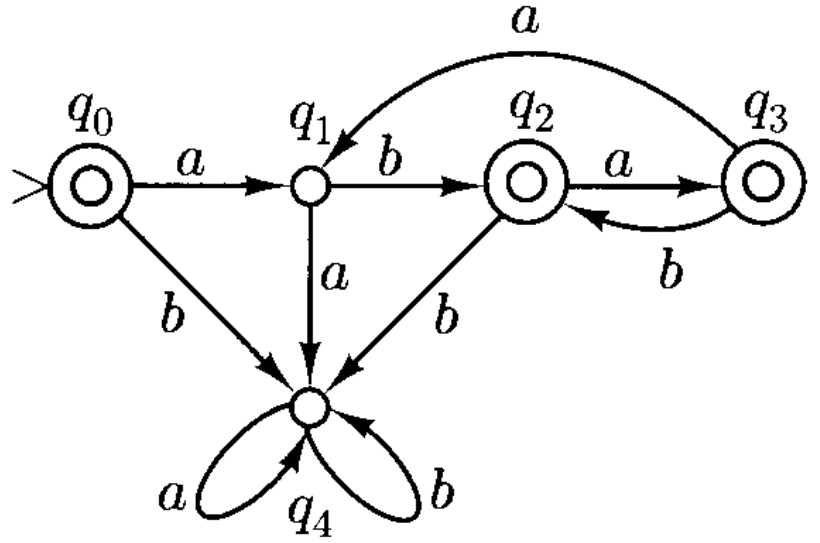
\includegraphics[width=.3\textwidth]{img/Fig2.4.png}
  \caption{}
\end{figure}

To see that a nondeterministic finite automaton can be a much more convenient device to design than a deterministic finite automaton, consider the language $L = (ab \cup aba)^*$, which is accepted by the deterministic finite automaton illustrated in Figure 3.

\begin{figure}[ht!]
  \centering
  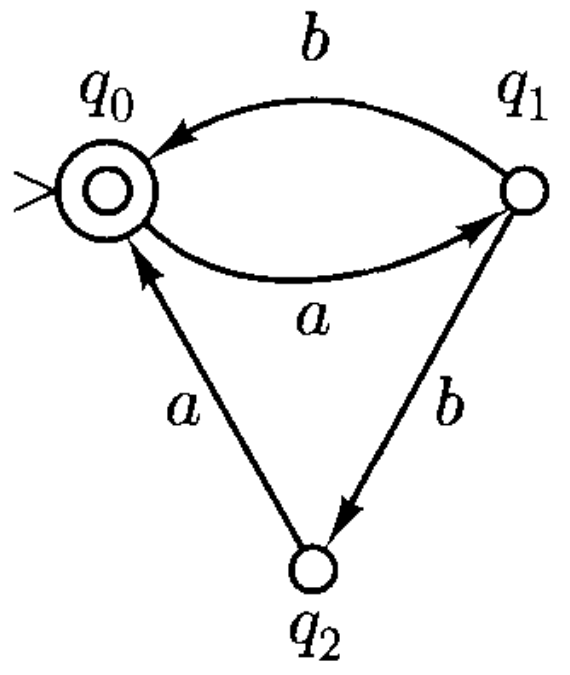
\includegraphics[width=.2\textwidth]{img/Fig2.5.png}
  \caption{}
\end{figure}

$L$ is accepted by the simple nondeterministic device shown in Figure 4. When this device is in state $q_l$ and the input symbol is $b$, there are two possible next states, $q_0$ and $q_2$. Thus Figure 4 does not represent a deterministic finite automaton.

\begin{figure}[ht!]
  \centering
  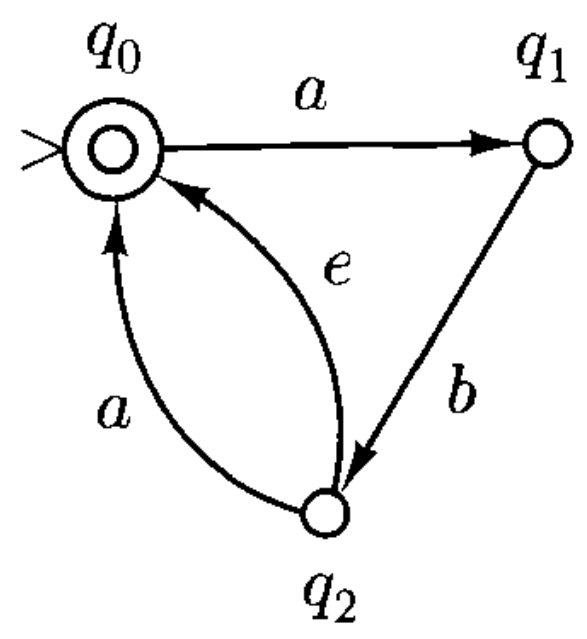
\includegraphics[width=.2\textwidth]{img/Fig2.6.png}
  \caption{}
\end{figure}

We also allow in the state diagram of a nondeterministic automaton arrows that are labeled by the empty string $e$. For example, the device of Figure 5 accepts the same language L. From q2 this machine can return to qo either by reading an $a$ or immediately, without consuming any input.

\begin{definition}{}
  A \textbf{nondeterministic finite automaton} is a quintuple $M = (K, \Sigma, \Delta, s, F)$, where
  \begin{itemize}
    \item $K$ is a finite set of \textbf{states}
    \item $\Sigma$ is an alphabet
    \item $s \in K$ is the \textbf{initial state}
    \item $F \subseteq K$ is the set of \textbf{final states}, and
    \item $\Delta$, the \textbf{transition relation}, is a subset of $K \times (\Sigma \cup \{e\}) \times K$ 
\end{itemize}
\end{definition}

$(q, a, p) \in \Delta$ is called a \textbf{transition} of $M$. $(q, e, p)$ indicates that the machine can pass to state $p$ from state $q$ without reading an input symbol.

\newpage
\begin{multicols}{2}
\setlength{\columnsep}{1.5cm}
\setlength{\columnseprule}{0.2pt}
  The configuration of the machine is the current state and the unread part of the input string, i.e., a configuration is an element of $K \times \Sigma^*$.\\

  The binary $\vdash_M$ (\textbf{yields}) relation holds between two configurations of $M$ if and only if the machine can pass from one configuration to another one as a result of a \textit{single move}. Let $(q, w)$ and $(q', w')$ be two configurations of $M$. Then $(q, w) \vdash_M (q', w')$ if and only if $w = aw'$ for some $a \in \Sigma \cup \{e\}$ and $(q, a, q') \in \Delta$. $(q, w) \vdash_M (q', w')$ reads $(q, w)$ \textbf{yields} $(q', w')$ \textbf{in one step}. Note that $\vdash_M$ might not be a function, i.e., there might be several pairs $(q', w')$ (or none at all) such that $(q, w) \vdash_M (q', w')$.\\

  $\vdash^*_M$ is the \textbf{reflexive transitive closure} of $\vdash_M$. $(q, w) \vdash^*_M (q', w')$ reads $(q, w)$ yields $(q', w')$. A string $w \in \Sigma^*$ is \textbf{accepted} by $M$ if and only if there is a state $f \in F$ such that $(s, w) \vdash^*_M (f, e)$. The \textbf{language} of $M$, $L(M)$, is the set of strings accepted by $M$.\\

  A deterministic finite state automaton is just a special type of nondeterministic finite state automaton. We obtain a DFA when $\Delta$ defines a function from $K \times \Sigma$ to $K$. In other words, an NFA $M = (K, \Sigma, \Delta, s, F)$ is deterministic if there are no transitions of the form $(q, e, p)$ and for each $q \in K$ and $a \in \Sigma$, there exists \textit{exactly one} $p \in K$ such that $(q, a, p) \in \Delta$.\\

  We can conclude that the class of languages recognized by deterministic finite state automaton is a \textit{subset} of the class of languages recognized by nondeterministic finite state automaton. Essentially, these classes are the same: A nondeterministic finite automaton can always be
  converted to an \textit{equivalent} deterministic finite state automaton.\\

  Two automaton $M_1$ and $M_2$ are said to be \textbf{equivalent} when $L(M_1) = L(M_2)$.
\end{multicols}

\begin{theorem}{}
  \textit{For each nondeterministic finite automaton, there exists an equivalent deterministic finite automaton.}
\end{theorem}

\begin{proof}
  The proof of the theorem is constructive: use \textbf{subset construction} algorithm to construct a DFA from an NFA and then show they are equivalent. Given an NFA $M = (K, \Sigma, \Delta, s, F)$, the algorithm constructs an equivalent DFA $M' = (K', \Sigma, \delta, s', F')$ as follows. For each state $q \in K$, the set of states that can be reached without reading an input symbol is defined as
  \begin{align*}
    E(q) = \left\{ p \in K\ |\ (q, e) \vdash^*_M (p, e) \right\}& &\textnormal{(Check Example 2)}
  \end{align*}
  Essentially, $E(q)$ is the reflexive transitive closure of the set $\left\{ q \right\}$ under the relation $\left\{(p, r)\ |\ (p, e, r) \in \Delta \right\}$. The DFA is defined as:
  \begin{align*}
    K' &= 2^K\\
    s' &= E(s)\\
    F' &= \left\{ Q \subseteq K\ |\ Q \cap F \neq \emptyset \right\}\\
    \delta'(Q, a) &= \left\{ E(p) : p \in K, (q, a, p) \in \Delta \textnormal{ for some } q \in Q \right\} \textnormal{ for each $Q \in K'$ and $a \in \Sigma$}\\
    &= \bigcup \left\{ E(p) : p \in K, (q, a, p) \in \Delta \textnormal{ for some } q \in Q \right\}
  \end{align*}
  To prove that $M$ and $M'$ are equivalent, show that for any string $w \in \Sigma^*$
  \begin{equation*}
    (s, w) \vdash^*_M (f, e) \textnormal{ for some } f \in F \textnormal{ iff } (E(s), q) \vdash^*_{M'} (P, e) \textnormal{ for some } P \in F'
  \end{equation*}
  Thus they recognize the same language.
\end{proof}

\begin{figure}[ht!]
  \centering
  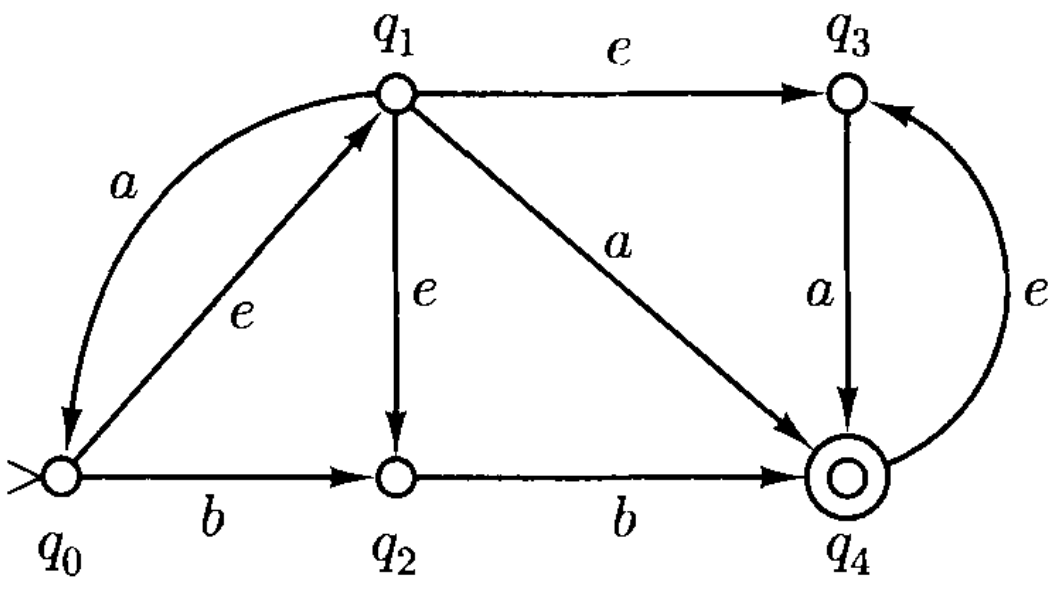
\includegraphics[width=.3\textwidth]{img/Fig2.9.png}
  \caption{}
\end{figure}

\begin{examplebreak}{}
  In the automaton of Figure 6, we have $E(q_0) = \left\{ q_0, q_1, q_2, q_3  \right\}$, $E(q_1) = \left\{ {q_1, q_2, q_3} \right\}$, $E(q_2) = \left\{ q_2 \right\}$, $E(q_3) = \left\{ q_3 \right\}$, and $E(q_4) = \left\{ q_3, q_4 \right\}$.
\end{examplebreak}


\begin{figure}[t]
  \centering
  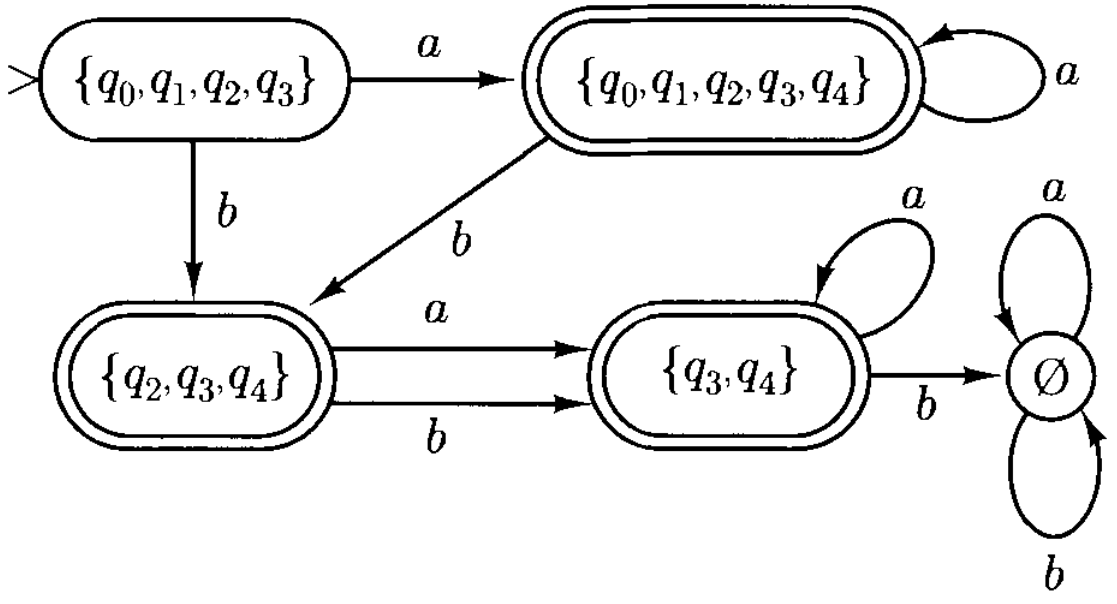
\includegraphics[width=.5\textwidth]{img/Fig2.10.png}
  \caption{}
\end{figure}


\begin{examplebreak}{: NFA to DFA}
  \quad Let's apply the algorithm then to the nondeterministic automaton in Figure 6. Since $M$ has 5 states, $M'$ will have $2^5 = 32$ states. However, only a few of these states will be relevant to the operation of $M'$ -namely, those states that can be reached from state $s'$ by reading some input string. Obviously, any state in $K'$ that is not reachable from $s'$ is irrelevant to the operation of $M'$ and to the language accepted by it. We shall build this reachable part of $M'$ by starting from $s'$ and introducing a new state only when it is needed as the value of $\delta'(q, a)$ for some state $q \in K'$ already introduced and some $a \in \Sigma$.
  
  \quad We have already defined $E(q)$ for each state $q$ of $M$ (from Example 2). Since $s' = E(q_0) = \left\{ q_0, q_1, q_2, q_3  \right\}$,
  \begin{equation*}
    (q_1, a, q_0),\ (q_1, a, q_4), \textnormal{ and } (q_3, a, q_4)
  \end{equation*}
  are all the transitions $(q, a, p)$ for some $q \in s'$. It follows that
  \begin{equation*}
    \delta'(s', a) = E(q_0) \cup E(q_4) = \left\{ q_0, q_1, q_2, q_3, q_4 \right\}
  \end{equation*}
  Similarly,
  \begin{equation*}
    (q_0, b, q_2) \textnormal{ and } (q_2, b, q_4)
  \end{equation*}
  are all the transitions of the form $(q, b, p)$ for some $q \in s'$, so
  \begin{equation*}
    \delta'(s', b) = E(q_2) \cup E(q_4) = \left\{ q_2, q_3, q_4 \right\}
  \end{equation*}
  Repeating this calculation for the newly introduced states, we have the following,,
  \begin{align*}
    \delta'(\left\{ q_0, q_1, q_2, q_3, q_4 \right\}, a) &= \left\{ q_0, q_1, q_2, q_3, q_4 \right\}\\
    \delta'(\left\{ q_0, q_1, q_2, q_3, q_4 \right\}, b) &= \left\{ q_2, q_3, q_4 \right\}\\
    \delta'(\left\{ q_2,q_3,q_4 \right\},a) &= E(q_4) = \left\{ q_3,q_4 \right\}\\
    \delta'(\left\{ q_2,q_3,q_4 \right\},b) &= E(q_4) = \left\{ q_3,q_4 \right\}
  \end{align*}
  Next,
  \begin{align*}
    \delta'(\left\{ q_3, q_4 \right\}, a) &= E(q_4) = \left\{ q_3, q_4 \right\}\\
    \delta'(\left\{ q_3, q_4 \right\}, b) &= 0
  \end{align*}
  and finally
  \begin{equation*}
    \delta'(\emptyset, a) = \delta'(\emptyset, b) = \emptyset
  \end{equation*}
  The relevant part of $M'$ is illustrated in Figure 7. $F'$, the set of final states, contains each set of states of which $q_4$ is a member, since $q_4$ is the sole member of $F$; so in the illustration, the three states $\left\{ q_0, q_1, q_2, q_3, q_4 \right\}$, $\left\{ q_2, q_3, q_4 \right\}$, and $\left\{ q_3,q_4 \right\}$ of $M'$ are final.
\end{examplebreak}

\textit{Basically, first look the initial state of NFA. E(s), a set, will be the initial state of DFA. It was $\left\{ q_0, q_1, q_2, q_3 \right\}$ for the example 3. Then look the each element of the set, if there is a way to any other state by reading an input inside alphabet (in example it is (a, b)), note that state(s) and combine their E(s'). In the first part of example $\delta'(s', a) = E(q_0) \cup E(q_4) = \left\{ q_0, q_1, q_2, q_3, q_4 \right\}$. When introduce new state, repeat that.}
